\documentclass[tikz,border=10pt]{standalone}
\usepackage{tikz}

\begin{document}

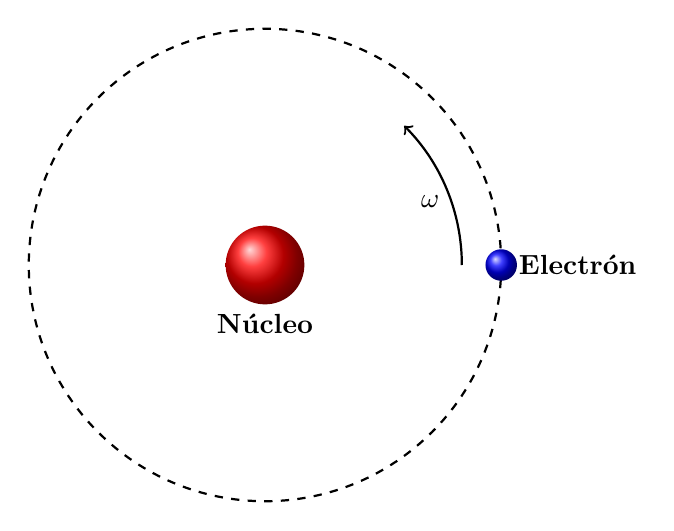
\begin{tikzpicture}
  % Nucleus
  \shade[ball color=red] (0,0) circle (0.5);
  \node[below] at (0,-0.5) {\textbf{Núcleo}};

  % Orbital
  \draw[thick,dashed] (0,0) circle (3);

  % Electron
  \shade[ball color=blue] (3,0) circle (0.2);
  \node[right] at (3.1,0) {\textbf{Electrón}};

  % Motion
  \draw[->,thick] (2.5,0) arc[start angle=0,end angle=45,radius=2.5];
  \node at (2.1,0.8) {$\omega$};
\end{tikzpicture}

\end{document}
